\documentclass[letterpaper,12pt,fleqn]{article}
\usepackage[margin=1in]{geometry}
\usepackage{libertine}
\usepackage{parskip}
\usepackage{enumitem}
\usepackage{amsfonts}
\usepackage{amssymb}
\usepackage{amsthm}
\usepackage{mathtools}
\usepackage{mathrsfs}
\usepackage{graphicx}
\pagestyle{plain}

\begin{document}   

\begin{center}
  \large
  \textbf{Spring 2020 Math 30 Makeup Final Exam}
\end{center}

\vspace{0.5in}

Name: \rule{4in}{1pt}

\vspace{0.5in}

\begin{enumerate}[left=0in]
\item Determine the limits:

  \vspace{0.5in}

  \begin{enumerate}
  \item \(\displaystyle\lim_{x\to-1^+}\frac{x^{5}-1}{x^{5}+1}\)

    \vspace{1in}

  \item \(\displaystyle \lim_{x\to +\infty}\arctan \frac{x^{10}-3x^5-2}{x^{10}+4x^3-1}\)

    \vspace{1in}

  \item \(\displaystyle \lim_{x\to e^+}\frac{1}{x \ln(x-1)}\)

    \vspace{1in}

  \item \(\displaystyle \lim_{x\to +\infty}\frac{2x}{(x-1)\ln x}\)
  \end{enumerate}

  \newpage

\item Using the limit definition of the derivative, find \(f'(x)\) where:
  \[f(x) = 6x^3 + 2x\]
  Show your work and \emph{do NOT use differentiation rules}.

  \newpage

\item You need to find the dimensions of a cylindrical can (much like a soda or soup can) so that its volume is 81
  cubic inches.  The metal used for the side of the can costs 50 cents per square inch, the metaul used for the
  bottom of the can costs 65 cents per square inch, and the metal used for the top of the can costs 85 cents per
  square inch.  Find the dimensions of the can that minimize the cost.  What is the minimum cost?  How do you know
  that your answer gives a minimum?

  \newpage

\item Find an equation for the tangent line to the curve:
  \[f(x)=3\sqrt{9x}-6e^{(2-x)}\]
  at \(x=2\).

  \newpage

\item Show all necessary steps:
  \begin{enumerate}
  \item Differentiate:
    \[g(x) = \arctan\sqrt{\sin x}\]

    \vspace{3in}

  \item Find the most general antiderivative of the function:
    \[f(x) = \dfrac{x^2+x+1}{x}\]
  \end{enumerate}

\item Two trains, the red train and the blue train, start at Wooster Station and travel to nearby towns.  The red
  train travels East at 40 mph while the blue train North at 60 mph.  The red train leaves at noon.  30 minutes
  later, the blue train leaves.  How fast is the distance between the two trains changing at 1 pm?

  \newpage

\item Find the following derivatives:
  \begin{enumerate}
  \item Find the first derivative:
    \[y=\sqrt[3]{x}\cdot\sec\sqrt{x}\]

    \vspace {3in}
  \item Find the second derivative:
    \[f(x)=\ln (3+x^4)\]
  \end{enumerate}

  \newpage

\item Find \(y'\):
  \[y=x^{x^2}\]

  \vspace{3in}

\item Find \(\frac{dy}{dx}\) at the point \((\frac{\pi}{4},\frac{\pi}{4})\) on the curve:
  \[2\cos x\sin y=1\]

  \newpage

\item The position of a particle moving along a coordinate axis is given by:
  \[s(t)=t^3-9t^2+24t+4\qquad t\ge 0\]

  \vspace{0.5in}

  \begin{enumerate}
  \item Find the velocity \(v(t)\).

    \vspace{2in}
    
  \item Find the acceleration \(a(t)\).

    \vspace{2in}
    
  \item Over what time intervals is the particle moving from left to right? From right to left?
  \end{enumerate}

  \newpage

\item Suppose that \(f(x)\) has the graph shown below.  Sketch the graph of \(f'(x)\).  Make sure that you clearly
  show any critical point(s) or asymptote(s).

  \begin{center}
    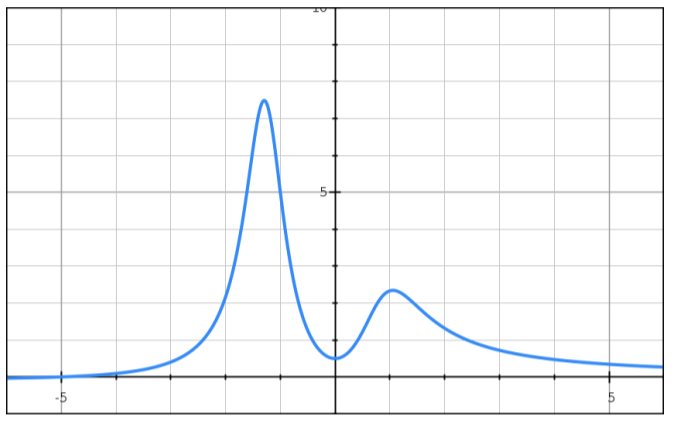
\includegraphics{graph1}
  \end{center}

  \newpage

\item Is it possible to sketch a graph that satisfies ALL of the following conditions?  If yes then sketch the graph of
  \(f\) below.  Otherwise, explain (in one or two sentences) why not.
  \begin{itemize}
  \item \(f(0)=0\)
  \item \(\displaystyle\lim_{x\to-4^-}f(x)=2\) and \(\displaystyle\lim_{x\to-4^+}f(x)=-2\)
  \item \(f\) is continuous from the left at \(x=-4\)
  \item \(f(x)\to\infty\) as \(x\to2^-\) and \(f(x)\to-\infty\) as \(x\to2^+\)
  \item \(f\) is continuous at all values of \(x\) other than \(x=-4\) and \(x=2\)
  \end{itemize}

  \newpage

\item Suppose that \(f(x)\) is a function whose derivative \(f'(x)\) is graphed below on the domain
  \(-3\leq x\leq 4\).

  \vspace{0.5in}

  \begin{center}
    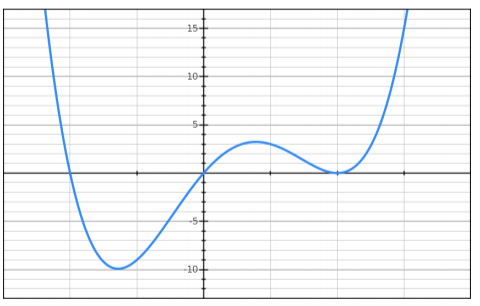
\includegraphics{graph2}
  \end{center}

  \vspace{0.5in}

  \begin{enumerate}
  \item Find the interval(s) where \(f\) is increasing and the interval(s) where \(f\) is decreasing.  Justify
    your answer.

    \vspace{2in}
    
  \item Find the \(x\) value of the relative/local maximum(s) of \(f\).  Justify your answer.

    \newpage
    
  \item Find the interval(s) of concavity of \(f\).  Justify your answer.

    \vspace{3in}
    
  \item Find the \(x\) value of the point(s) of inflection of \(f\).  Justify your answer.
  \end{enumerate}
\end{enumerate}

\end{document}
